\documentclass[11pt]{article}
\usepackage[margin = 1in]{geometry}
\usepackage{amsmath}
\usepackage{amssymb}
\usepackage{amsthm}
\usepackage{graphicx}
\usepackage{enumitem}
\usepackage{url}
\usepackage[parfill]{parskip}
\usepackage{listings}
\newcommand{\skipline}{\vspace{\baselineskip}}
\newcommand{\spacer}{\noalign{\medskip}}
\newcommand{~}{\sim}
\newenvironment{problem}[1]{\textbf{Problem #1: }}{\newpage}
\usepackage{caption}
\usepackage{subcaption}
\usepackage[utf8]{inputenc}
\usepackage{xcolor}
\definecolor{codegreen}{rgb}{0,0.6,0}
\definecolor{codegray}{rgb}{0.5,0.5,0.5}
\definecolor{codepurple}{rgb}{0.58,0,0.82}
\definecolor{backcolour}{rgb}{0.95,0.95,0.92}
\lstdefinestyle{mystyle}{
	backgroundcolor=\color{backcolour},   
	commentstyle=\color{codegreen},
	keywordstyle=\color{magenta},
	numberstyle=\tiny\color{codegray},
	stringstyle=\color{codepurple},
	basicstyle=\ttfamily\footnotesize,
	breakatwhitespace=false,         
	breaklines=true,                 
	captionpos=b,                    
	keepspaces=true,                 
	numbers=left,                    
	numbersep=5pt,                  
	showspaces=false,                
	showstringspaces=false,
	showtabs=false,                  
	tabsize=2
}
\lstset{style=mystyle}
\usepackage{MnSymbol}
\usepackage{pdfpages}

\begin{document}
	
	\begin{center}
		\textbf{Assignment 5} \\
		\textbf{Computer Vision} \\
		\textbf{CS 559} \\
		\textbf{Stephen Giang RedID: 823184070} \\
		\skipline \skipline
	\end{center}

	\begin{problem}{1}
		Suppose that the boundary of a closed region is represented by a 4-directional chain code.  Write a function Area(ChainCode) in pseudo-code to compute the area of the region from its chain code representation.
		\\ \\
		Notice, we can find the area enclosed by a chain code using the area of a polyline:
		\[A = \frac{1}{2} \sum_{i = 0}^{n - 1}\left(x[i + 1]y[i] - x[i]y[i+1]\right)\]
		Now we can let the following:
		\begin{enumerate}[label = (\roman*)]
			\item Let the starting point be notated as $(x_0, y_0) = (0,0)$
			\item Let 1 be up, 2 be left, 3 be down, and 0 be right
			\item Let ChainCode be an array consisting of the following numbers: \{0,1,2,3\}
		\end{enumerate}
		Notice the code below: \\
\begin{lstlisting}[language=Matlab]
function A = Area(ChainCode) 

	xarr = zeros(length(ChainCode) + 1);
	yarr = zeros(length(ChainCode) + 1); 
	
	% convert ChainCode into polyline
	x = 0; y = 0;
	pointIndex = 2;
	for i = 1 : length(ChainCode)
		if (ChainCode(i) == 1), y = y + 1;
		elseif (ChainCode(i) == 2), x = x - 1;
		elseif (ChainCode(i) == 3), y = y - 1;
		elseif (ChainCode(i) == 0), x = x + 1; 
		end
		xarr(pointIndex) = x;
		yarr(pointIndex) = y;
		pointIndex = pointIndex + 1;
	end
	
	% Shoelace Formula
	sum = 0;
	for i = 1 : length(ChainCode)
		sum = sum + ((xarr(i + 1) * yarr(i)) - (xarr(i) * yarr(i + 1)));
	end
	A = abs(sum) / 2;  

end
\end{lstlisting}
		
	\end{problem}

	\begin{problem}{2}
		Show that the area enclosed by the polyline $(x_0, y_0), (x_1, y_1), \cdots (x_{n-1}, y_{n-1}), (x_0, y_0)$ is given by
		\[A = \frac{1}{2} \sum_{i = 0}^{n - 1}\left(x[i + 1]y[i] - x[i]y[i+1]\right)\]
		\begin{proof}
			Notice, we can take the area of any simple closed loop from the following equation:
			\[A = \iint\limits_D dA = \iint\limits_D \left(\frac{dQ}{dx} - \frac{dP}{dy}\right)dA, \qquad \text{with $\left(\frac{dQ}{dx} - \frac{dP}{dy}\right) = 1$}\]
			Let the following be true:
			\[\frac{dQ}{dx} = \frac{1}{2}, \qquad Q = \frac{1}{2}x, \qquad \frac{dP}{dy} = \frac{-1}{2}, \qquad P = \frac{-1}{2}y\]
			Now we can use Green's theorem to say the following:
			\[A = \iint\limits_D \left(\frac{dQ}{dx} - \frac{dP}{dy}\right)dA = \rcircleleftint_C\, Q\,dy + P\,dx = \rcircleleftint_C\, \frac{1}{2}x\,dy - \frac{1}{2}y\,dx  = \frac{1}{2}\rcircleleftint_C\,  x\,dy -y\,dx\]
			We now take two points $(x_0, y_0), (x_1, y_1)$.  We can parameterize the line segment between the two points into:
			\[\vec{r}(t) = \langle\,\, (1 - t)x_0 + tx_1, (1 - t)y_0 + ty_1 \,\,\rangle\] 
			Notice the line integral between two points from the following equation:
			\begin{align*}
				\rcircleleftint_C  x\,dy -y\,dx &= \int_{t = 0}^{t = 1} \left((1 - t)x_0 + tx_1\right)(-y_0 + y_1) - \left((1 - t)y_0 + ty_1\right)(-x_0 + x_1)   \\
				&=\int_{t = 0}^{t = 1} -(1 - t)x_0y_0 + (1-t)x_0y_1 - tx_1y_0 + tx_1y_1  \\
				&\hspace{4em}+ (1-t)x_0y_0 - (1-t)x_1y_0 + tx_0y_1 - tx_1y_1 \\
				&= \int_{t = 0}^{t = 1}  (1-t)x_0y_1 - tx_1y_0 - (1-t)x_1y_0 + tx_0y_1  \\
				&= tx_0y_1 - \frac{t^2}{2}x_0y_1 - \frac{t^2}{2}x_1y_0 - tx_1y_0 + \frac{t^2}{2}x_1y_0 + \frac{t^2}{2}x_0y_1 \Bigg|_{t=0}^{t=1} \\
				&= tx_0y_1 - tx_1y_0  \Bigg|_{t=0}^{t=1} \\
				&=-(x_1y_0 -  x_0y_1) 
			\end{align*}
			Because when parametricizing  with $\vec{r}(t)$, we have that integral is taken in the counter clockwise order, however, the vertices are read in clockwise order in the shoelace formula, so we get:
			\[\lcirclerightint_C x\,dy -y\,dx = -\rcircleleftint_C  x\,dy -y\,dx = x_1y_0 -  x_0y_1 \]
			Now we get the following:
			\begin{align*}
				A = \frac{1}{2}\lcirclerightint_C\,  x\,dy -y\,dx = \frac{1}{2}\sum_{i = 0}^{n-1}\lcirclerightint_{C_i} x\,dy -y\,dx = \frac{1}{2} \sum_{i = 0}^{n - 1}\left(x_{i+1}y_i - x_iy_{i+1}\right)  = \frac{1}{2} \sum_{i = 0}^{n - 1}\left(x[i + 1]y[i] - x[i]y[i+1]\right)
			\end{align*}
			where $C_i$ for $i \in \{0,1,2,\cdots, n -2, n-1\}$ are the line segments between each vertex $(x_0, y_0), (x_1, y_1)$, $\cdots (x_{n-1}, y_{n-1}), (x_n = x_0, y_n = y_0)$ \\
		\end{proof}
	\end{problem}

	\begin{problem}{3}
		Compare Hough transform and Canny edge detection for region detection in terms of (i) robustness (insensitivity) to noise, (ii) detection of regions with irregular shape, (iii) any common technique that is used both methods. 
		\begin{enumerate}[label = (\roman*)]
			\item robustness (insensitivity) to noise
			\\ \\
			When it comes to noise, the Canny edge detector uses a Gaussian filter to remove as much noise as possible.  The noise reduction however can create disconnections of the edges so the edge detector uses a low and high threshold to refill the disconnections created.  If a certain pixel is in between the thresholds, it checks if the neighbor pixels have a high magnitude and if so, it makes it white, or makes it an edge pixel, otherwise it makes it black.
			\\ \\
			When it comes to noise, the Hough Transform uses an accumulator array.  For noise reduction, neighbor elements in the accumulator array are increased.
			\item detection of regions with irregular shape
			\\ \\
			When it comes to detection of regions with irregular shape, the Canny edge detector will have some trouble.  Because the detector is dependent on the neighboring pixels, an irregular shape will show irregular neighborhoods, which will make edge detection a lot harder. 
			\\ \\
			When it comes to detection of regions with irregular shape, the shape shouldn't matter with the Hough transform, because it simply takes in all the pixels and transforms it to a polar plane. Here the detection is not dependent on the shape, just simply the pixel coordinates or locations.
			\item any common technique that is used both methods
			\\ \\
			A common technique both share is that they both find the edges so that they can create a region to search and group.  This will make separating regions much easier.
		\end{enumerate}
	\end{problem}
	
	\begin{problem}{4}
		\begin{enumerate}[label = (\alph*)]
			\item Compare three losses compressions techniques in terms of their suitability for natural images. 
			\\ \\
			Notice the following three losses compressions techniques and their compression ratios for natural images:
			\begin{enumerate}[label = (\alph*)]
				\item Delta / Differential Coding - 1.8 : 1 ratio
				\item Run Length Encoding - 1.1 : 1 ratio
				\item Huffman Coding - 1.6 : 1 ratio
			\end{enumerate} 
			\item Explain which lossless compression technique use variable code length. Which technique results in the optimal code length?
			\\ \\
			The Huffman Coding lossless compression technique uses variable code length.  This is because in this technique, the codewords are chosen such that $L_{ave}$ is as close as possible to E, the measure for average number of bits per pixels.  Allowing us to choose our codewords giving us a variable code length.  Also because of this variable code length, we can make the code have a minimal code length this resulting in the optimal code length. 
		\end{enumerate}
	\end{problem}

	\begin{problem}{5}
		Consider the 8 by 8 subimage 
		\[f(x,y) = \begin{bmatrix}
			56 & 45 & 51 & 66 & 70 & 61 & 64 & 73 \\
			63 & 59 & 56 & 90 & 109 & 85 & 69 & 72 \\
			62 & 59 & 68 & 103 & 144 & 104 & 66 & 73 \\
			63 & 58 & 71 & 132 & 134 & 106 & 70 & 69 \\
			65 & 61 & 68 & 114 & 116 & 82 & 68 & 70 \\
			79 & 65 & 60 & 67 & 77 & 68 & 58 & 75 \\
			85 & 71 & 54 & 59 & 55 & 61 & 65 & 73 \\
			87 & 79 & 69 & 58 & 65 & 66 & 78 & 94
		\end{bmatrix}\]
		Apply the JPEG compression algorithm and find and report the 1-D coefficient sequence.
		\\ \\
		Notice the intermediate steps:
		\[\bar{f} = f - 128 = 
		\begin{bmatrix}
			-72 &	-83 &	-77 &	-62 &	-58 &	-67 &	-64 &	-55 \\
			-65 &	-69 &	-72 &	-38 &	-19 &	-43 &	-59 &	-56 \\
			-66 &	-69 &	-60 &	-25 &	 16 &	-24 &	-62 &	-55 \\
			-65 &	-70 &	-57 &	  4 &	 6  &	-22 &	-58 &	-59 \\ 
			-63 &	-67 &	-60 &	-14 &	-12 &	-46 &	-60 &	-58 \\
			-49 &	-63 &	-68 &	-61 &	-51	&   -60 &	-70 &	-53 \\
			-43 &	-57 &	-74 &	-69 &	-73 &	-67 &	-63 &	-55 \\ 
			-41 &	-49 &	-59 &	-70 &	-63 &	-62 &	-50 &	-34 \\
		\end{bmatrix}\]
		\[\bar{C}(u,v) = \begin{bmatrix}
			-426.125 & -28.938 & -55.423 & 27.216 & 56.625 & -13.318 & -4.779 & -3.264  \\ 
			7.489 & -26.110 & -60.683 & 11.661 & 15.989 & -4.170 & -3.059 & 1.695  \\ 
			-50.180 & 4.038 & 77.060 & -12.952 & -23.200 & 2.573 & 3.456 & 6.595  \\ 
			-47.261 & 9.686 & 29.100 & -11.038 & -4.090 & 10.161 & 0.527 & -2.266  \\ 
			9.375 & -6.109 & -9.619 & -12.588 & 2.125 & 11.001 & -2.645 & -3.143  \\ 
			-11.518 & 1.983 & 1.988 & 2.034 & -2.147 & 5.493 & 4.075 & -5.367  \\ 
			-1.268 & -3.184 & 5.206 & -0.291 & -0.808 & -10.021 & 7.940 & 9.357  \\ 
			-2.772 & -0.432 & -3.038 & -0.277 & 1.154 & -2.056 & -3.032 & 4.655   
		\end{bmatrix}\]
		\[C_q(u,v) = \begin{bmatrix}
			-27 & -3 & -6 & 2 & 2 & 0 & 0 & 0  \\ 
			1 & -2 & -4 & 1 & 1 & 0 & 0 & 0  \\ 
			-4 & 0 & 5 & -1 & -1 & 0 & 0 & 0  \\ 
			-3 & 1 & 1 & 0 & 0 & 0 & 0 & 0  \\ 
			1 & 0 & 0 & 0 & 0 & 0 & 0 & 0  \\ 
			0 & 0 & 0 & 0 & 0 & 0 & 0 & 0  \\ 
			0 & 0 & 0 & 0 & 0 & 0 & 0 & 0  \\ 
			0 & 0 & 0 & 0 & 0 & 0 & 0 & 0 
		\end{bmatrix}\]
		\\ 
		\[C_{q \{1D\}} = \begin{array}{cccccccccc}
			[ -27 & -3 & 1 & -4 & -2 & -6 & 2 & -4 & 0 & \cdots  \\ 
			-3 & 1 & 1 & 5 & 1 & 2 & 0 & 1 & -1 & \cdots \\ 
		    1 & 0 & 0 & 0 & 0 & 0 & 0 & -1 & \text{EOB} ]
		\end{array}\]
		\newpage
\begin{lstlisting}[language=Matlab]
% Quantization Table 
q = [16 11 10 16 24 40 51 61;
12 12 14 19 26 58 60 55;
14 13 16 24 40 57 69 56;
14 17 22 29 51 87 80 62;
18 22 37 56 68 109 103 77;
24 35 55 64 81 104 113 92;
49 64 78 87 103 121 120 101;
72 92 95 98 112 100 103 99;];

% Given Matrix
f = [56  45  51  66  70  61  64  73 ;
63  59  56  90  109  85  69  72 ;
62  59  68  103  144  104  66  73 ;
63  58  71  132  134  106  70  69 ;
65  61  68  114  116  82  68  70 ;
79  65  60  67  77  68  58  75 ;
85  71  54  59  55  61  65  73 ;
87  79  69  58  65  66  78  94];

% Step 1: bar{f} = f - 128
fb = f - 128;

% Step 2: Use DCT to get bar{C}
n = 8; Cb = zeros(8,8);
for u = 0 : (n - 1)
	for v = 0 : (n - 1)
		if (u == 0), a = sqrt(1 / n);
		else, a = sqrt(2 / n); end
	
		if (v == 0), b = sqrt(1 / n);
		else, b = sqrt(2 / n); end
	
		sum = 0;
		for x = 0 : (n - 1)
			for y = 0 : (n - 1)
				sum = sum + fb((x + 1), (y + 1))*cos((pi * (2*x + 1)* u) / (2*n)) * ...
				cos((pi * (2*y + 1)* v) / (2*n));
			end
		end
	
		Cb((u + 1), (v + 1)) = a*b*sum;
	end
end

% Step 3: Quantize bar{C}
Cq = round( Cb ./ q);
\end{lstlisting}
\newpage
\begin{lstlisting}[language=Matlab]
% Step 4: Arrange into 1D sequence in zig zag order
Cq1 = zeros(1,64);

i = 1; x = 1; y = 1; % Start
Cq1(i) = Cq(x, y);
i = i + 1; y = y + 1; % Right
while (i <= 64  )
	while (x >= 1 && y >= 1 && x <= 8 && y <= 8)
		Cq1(i) = Cq(x,y);
		i = i + 1;
		x = x + 1; % Down
		y = y - 1; % Left
	end
	if (x > 8)
		x = x - 1; % Up
		y = y + 1; % Right 
	end
	y = y + 1; % Right
	while (x >= 1 && y >= 1 && x <= 8 && y <= 8)
		Cq1(i) = Cq(x,y);
		i = i + 1;
		x = x - 1; % Up
		y = y + 1; % Right
	end
	if (y > 8)
		x = x + 1; % Down
		y = y - 1; % Left 
	end
	x = x + 1; % Down
end

% Remove trailing zeros
len = 64;
while (Cq1(len) == 0)
	len = len - 1;
end

Cq1 = Cq1(1 : len);
\end{lstlisting}
	\end{problem}

	\begin{problem}{6 (All Code on Last Pages)}
		Use the region growing function (next page) to detect:
		\begin{enumerate}[label = (\alph*)]
			\item The red, blue, green regions in the ThreeRegions image by planting one seed in each region simultaneously. You must run the program only once to detect all three regions. This requires just a little modification to the attached function.
			\\ \\
			For this, I simply modified the code such that it takes in a colored image, 3 seeds, and 3 maximum region distances.
			\begin{figure}[h!]
				\centering
				\begin{subfigure}{.45\textwidth}
					\centering
					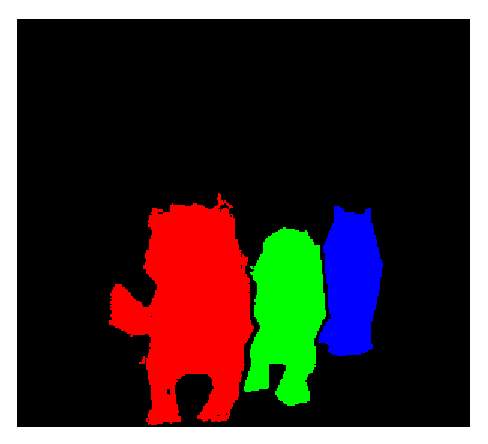
\includegraphics[height = 6cm]{Figures/Prob6a}
				\end{subfigure}
				\begin{subfigure}{.45\textwidth}
					\centering
					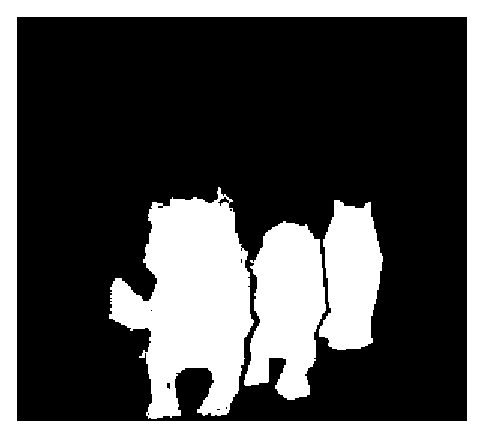
\includegraphics[height = 6cm]{Figures/Prob6a2}
				\end{subfigure}
			\end{figure}
			\item Determine the centroid, area, and circularity of the regions detected in (a)
			\\ \\
			For the area, I simply added the red, green, and blue components to get a single black and white matrix.  Because this matrix consisted of all 1's and 0's, I added the values of each pixel to count the number of pixels in the region as pixels in the region will be valued at 1 and 0 otherwise. 
			\[\text{Area: } A = 15246\]
			For the centroid, I got the following:
			\[x_c = \frac{1}{A}\sum_{x=0}^{w-1}\sum_{y=0}^{h-1}xf(x,y) = 183.35 \qquad y_c = \frac{1}{A}\sum_{x=0}^{w-1}\sum_{y=0}^{h-1}yf(x,y) = 149.63\]
			For the circularity, I got all the boundary points by using the canny edge detection.  Then I stored the location of all the pixels with values of 1 as they are the edge points.  Then I found the distance from each point to the centroid to get $d_i$.  Then I took the mean to get $d_{\text{ave}}$.  From there, I took the standard deviation to get $\sigma$.
			\[d_{\text{ave}} = \frac{1}{m}\sum_{i = 0}^{m-1} d_i = 61.35, \qquad \sigma = \sum_{i = 0}^{m-1} (d_i - d_{\text{ave}})^2 = 605569.1\]
			\newpage
			\item Detect the boundary of the region containing the red beans that are located in the center of the Beans image. Note that function does not know the location of beans, and only know the features of a single bean, say color and shape of it. This will need some modification to the function.
			\\ \\
			For this, I simply inputted a RGB color matrix, \textit{ie} [.64 .27 .29], and looped through the program to find that color.  Once found, that pixel would be the seed and it would run like part (a).
			\begin{figure}[h!]
				\centering
				\begin{subfigure}{.45\textwidth}
					\centering
					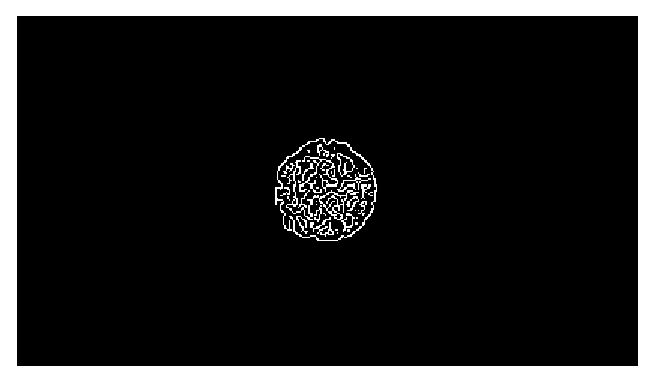
\includegraphics[height = 4.25cm]{Figures/Prob6c1}
				\end{subfigure}
				\begin{subfigure}{.45\textwidth}
					\centering
					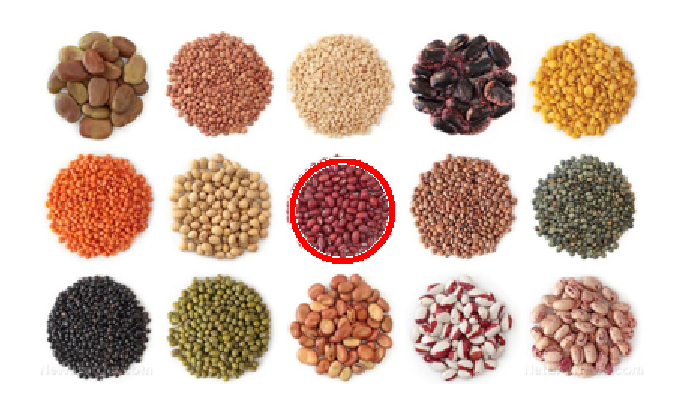
\includegraphics[height = 4.25cm]{Figures/Prob6c}
				\end{subfigure}
			\end{figure}
			\item Find the minimum distance between regions containing the red beans and the yellow ( in the upper right corner) of the image. Again the function does not know the locations of these two regions.
			\\ \\
			After finding the circle boundaries over each bean pile found using the function from part (c), I now have the center and radius of each circle. 
			\\ \\
			Notice the following:
			\[C_1 = (201.4, 115.6), \qquad C_2 = (356.1, 36.6), \qquad r_1 = 32.1, \qquad r_2 = 33.4\]
			To get the minimum distance, all we need to do is take the distance between the centers and subtract the two radii. Notice the following:
			\begin{align*}
				d_{\text{min}} &= \sqrt{(x_{C2} - x_{C_1})^2 + (y_{C2} - y_{C_1})^2} - (r_1 + r_2)\\
				&= \sqrt{(356.1 - 201.4)^2 + (36.6 - 115.6)^2} - (32.1 + 33.4) \\
				&= 108.1923 \text{ pixels}
			\end{align*}
			\begin{figure}[h!]
				\centering
				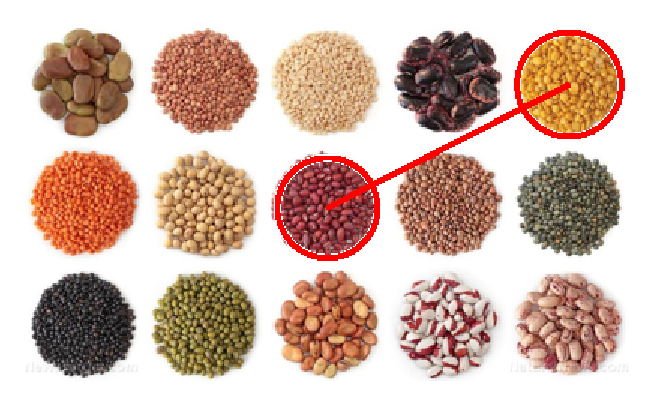
\includegraphics[height = 4.25cm]{Figures/Prob6d}
			\end{figure}
			\newpage
\begin{lstlisting}[language=Matlab]
function J = regiongrowing(I,x,y,reg_maxdist)
%
% This function performs "region growing" in an image from a specified
% seedpoint (x,y)
%
% J = regiongrowing(I,x,y,t) 
% 
% I : input image 
% J : logical output image of region
% x,y : the position of the seedpoint (if not given uses function getpts)
% t : maximum intensity distance (defaults to 0.2)
%
% The region is iteratively grown by comparing
% all unallocated neighbouring pixels to the region.
% The difference between a pixel's intensity value and the region's mean, 
% is used as a measure of similarity. The pixel with the smallest difference 
% measured this way is allocated to the respective region. 
% This process stops when the intensity difference between region mean and
% new pixel become larger than a certain treshold (t)
%
% Example:
%
% I = im2double(imread('medtest.png'));
% x = 198; y = 359;
% J = regiongrowing(I,x,y,0.2); 
% figure, imshow(I+J);
%
% Author: D. Kroon, University of Twente
%
	
	if(exist('reg_maxdist','var') == 0) 
		reg_maxdist = 0.2; 
	end
	
	if(exist('y','var') == 0) 
		figure, imshow(I,[]); 
		[y,x] = getpts; 
		y = round(y(1)); x = round(x(1)); 
	end
	
	J = zeros(size(I));     % Output 
	Isizes = size(I);       % Dimensions of input image
	reg_mean = I(x,y);      % The mean of the segmented region
	reg_size = 1;           % Number of pixels in region
	
	% Free memory to store neighbours of the (segmented) region
	neg_free = 10000; neg_pos=0;
	neg_list = zeros(neg_free,3); 
	pixdist = 0;  % Distance of the region newest pixel to the regio mean
	
	% Neighbor locations (footprint)
	neigb = [-1 0; 1 0; 0 -1;0 1];
\end{lstlisting}
\newpage
\begin{lstlisting}[language = Matlab]
	% Start regiogrowing until distance between regio and posible new pixels 
	% become higher than a certain treshold
	while(pixdist < reg_maxdist && reg_size < numel(I))
	
		% Add new neighbors pixels
		for j = 1 : 4
			% Calculate the neighbour coordinate
			xn = x + neigb(j,1); yn = y +neigb(j,2);
			
			% Check if neighbour is inside or outside the image
			ins = (xn >= 1) && (yn >= 1) && (xn <= Isizes(1)) && (yn <= Isizes(2));
			
			% Add neighbor if inside and not already part of the segmented area
			if(ins && (J(xn,yn) == 0)) 
				neg_pos = neg_pos+1;
				neg_list(neg_pos,:) = [xn yn I(xn,yn)]; J(xn,yn)=1;
			end
		end
		
		% Add a new block of free memory
		if(neg_pos + 10 > neg_free) 
			neg_free = neg_free + 10000; 
			neg_list((neg_pos + 1):neg_free , :)=0; 
		end
		
		% Add pixel with intensity nearest to the mean of the region, to the region
		dist = abs(neg_list(1:neg_pos,3) - reg_mean);
		[pixdist, index] = min(dist);
		J(x,y) = 2; reg_size = reg_size + 1;
		
		% Calculate the new mean of the region
		reg_mean = ( reg_mean*reg_size + neg_list(index,3) ) /(reg_size+1);
		
		% Save the x and y coordinates of the pixel (for the neighbour add proccess)
		x = neg_list(index,1); y = neg_list(index,2);
		
		% Remove the pixel from the neighbour (check) list
		neg_list(index,:) = neg_list(neg_pos,:); 
		neg_pos = neg_pos-1;
	end
	
	% Return the segmented area as logical matrix
	J = J > 1;
end
\end{lstlisting}
		\newpage
		\end{enumerate}
	\includepdf[pages=-]{Code/Prob6}
	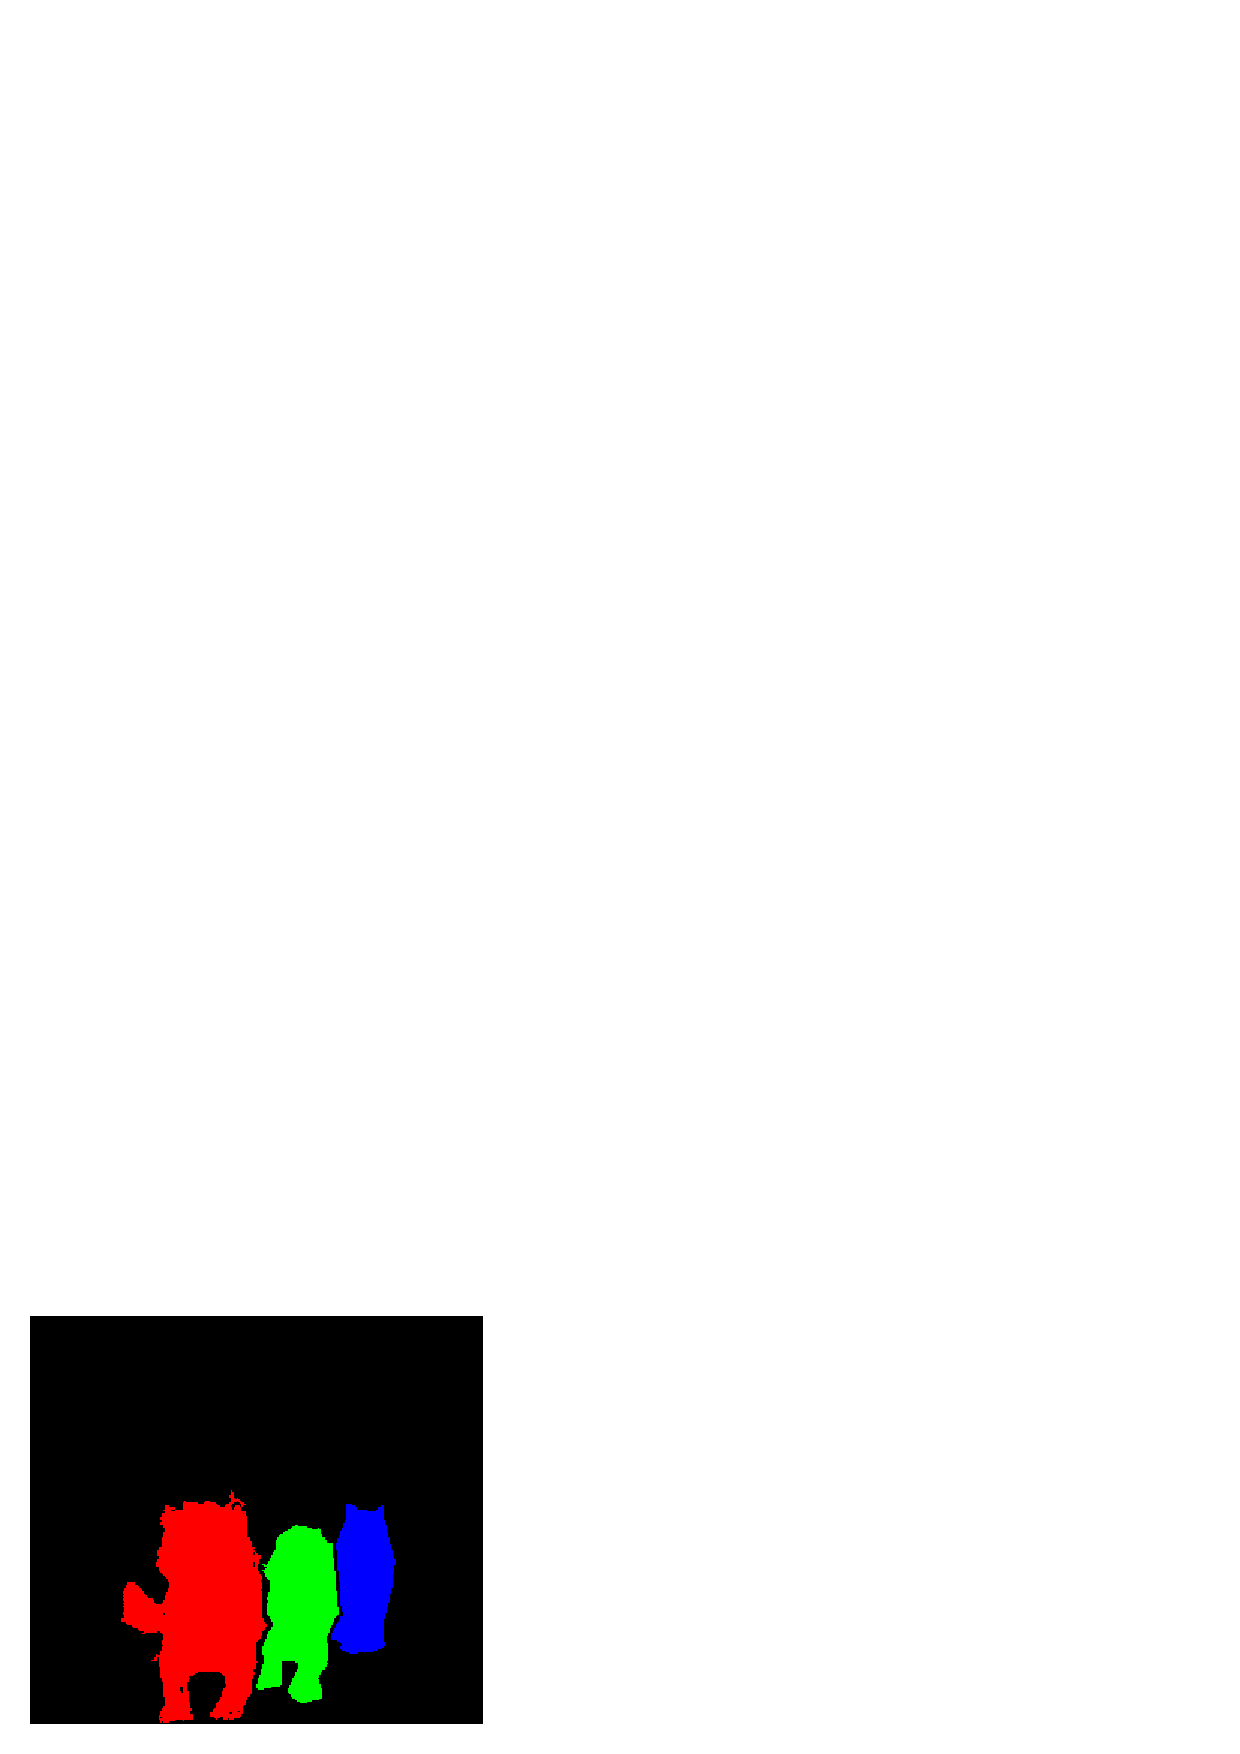
\includepdf[pages=-]{Code/Prob6a}
	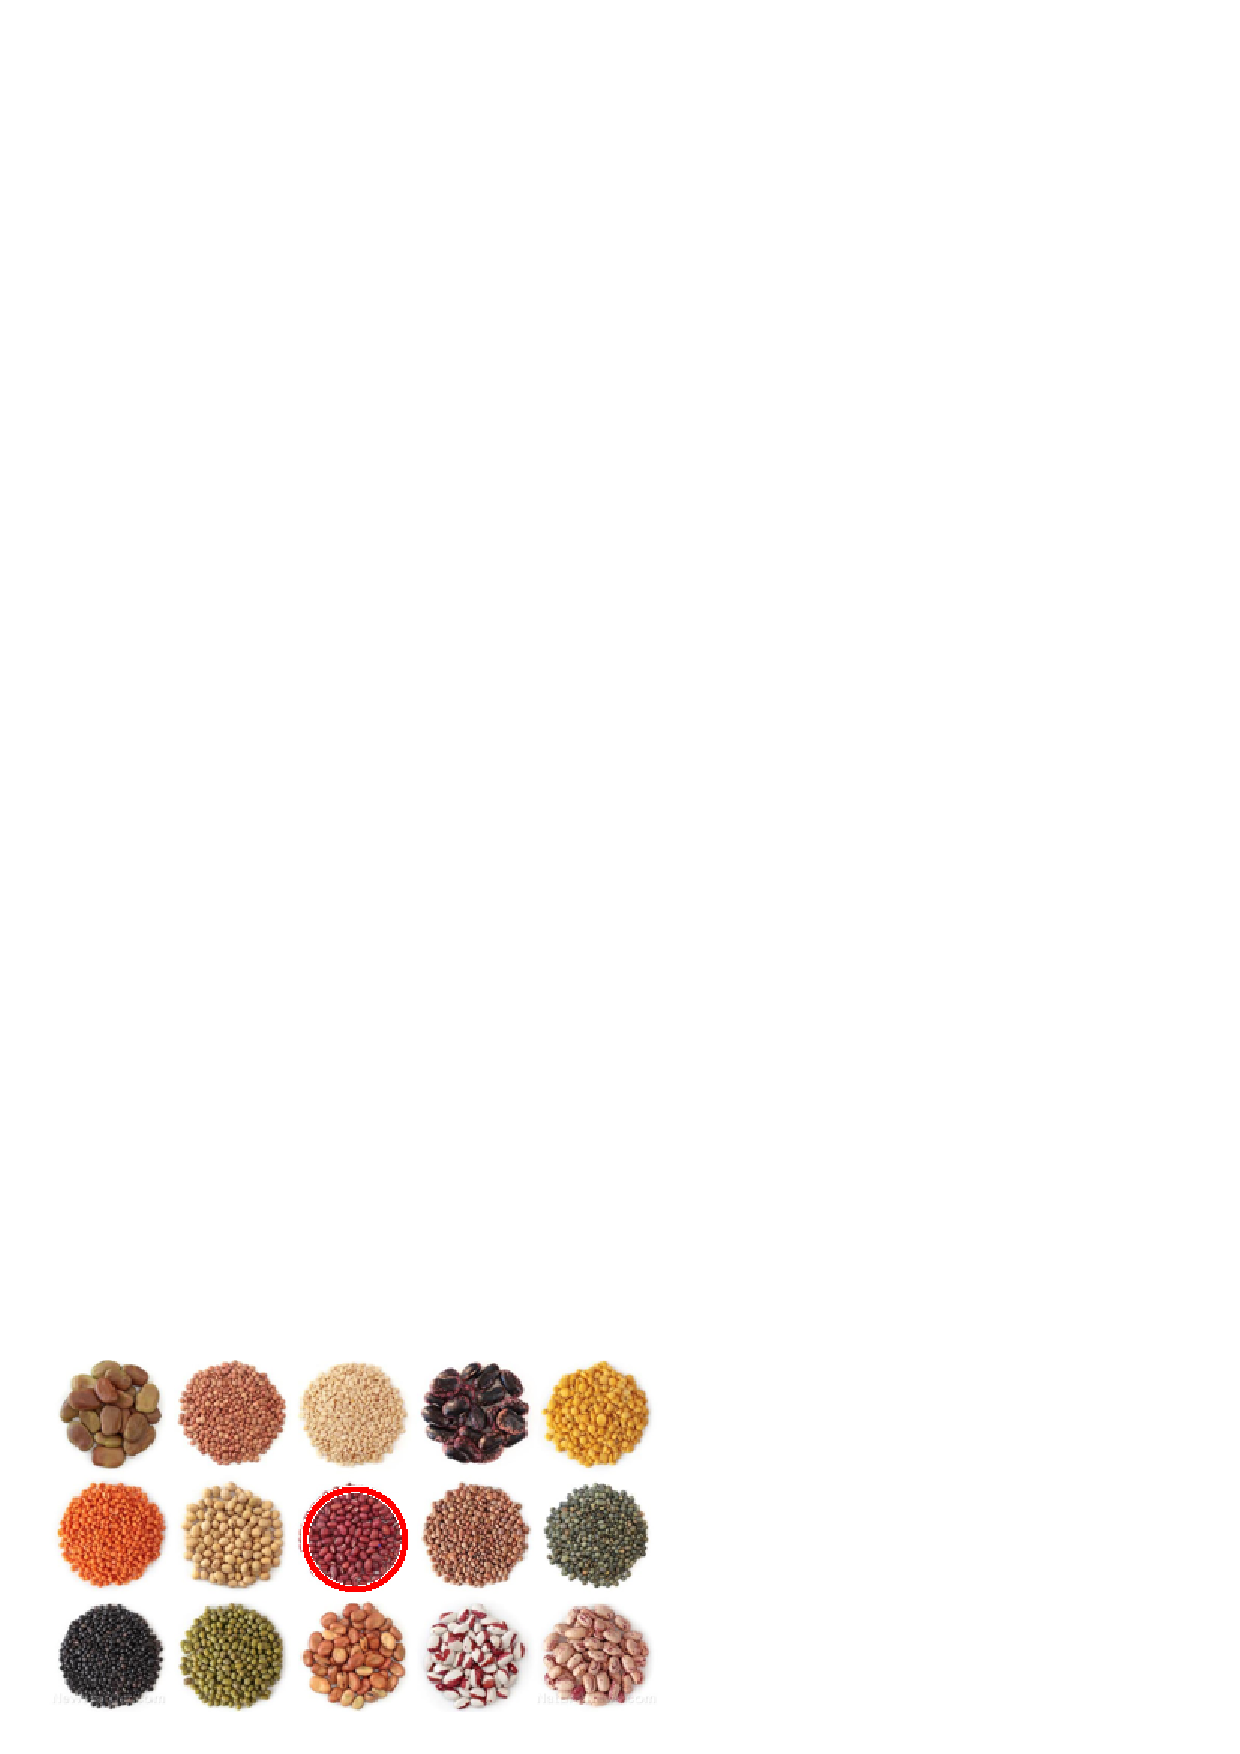
\includepdf[pages=-]{Code/Prob6c}
	\end{problem}


\end{document}
